\section{Filtros Pasaaltos}
Se simularon los siguientes filtros pasaaltos con sus respectivas ventanas en MATLAB.

\begin{table}[H]
\centering
\begin{tabular}{|c|c|c|c|c|c|}
\hline
$f_s(Hz)$ & $f_p(Hz)$ & $f_a(Hz)$ & $A_p(dB)$ & $A_a(dB)$ & Ventana     \\ \hline
$44.1k$   & $1k$      & $2k$      & 2         & 20        & Rectangular \\
$44.1k$   & $1k$      & $2k$      & 2         & 40        & Hamming     \\
$44.1k$   & $1k$      & $2k$      & 1         & 40        & Blackman    \\
$44.1k$   & $2.4k$    & $3.6k$    & 2         & 40        & Kaiser      \\
$44.1k$   & $1k$      & $2k$      & 2         & 60        & Kaiser      \\ \hline
\end{tabular}
\caption{Plantillas de filtros pasaaltos realizados.}
\label{tab:plantillaspasaaltos}
\end{table}

\subsection{Ventana Rectangular}
La ventana rectangular está definida por:
\begin{equation}
    \omega (n+1)=1 \qquad  0<n<N-1
\end{equation}
\begin{figure}[H]
  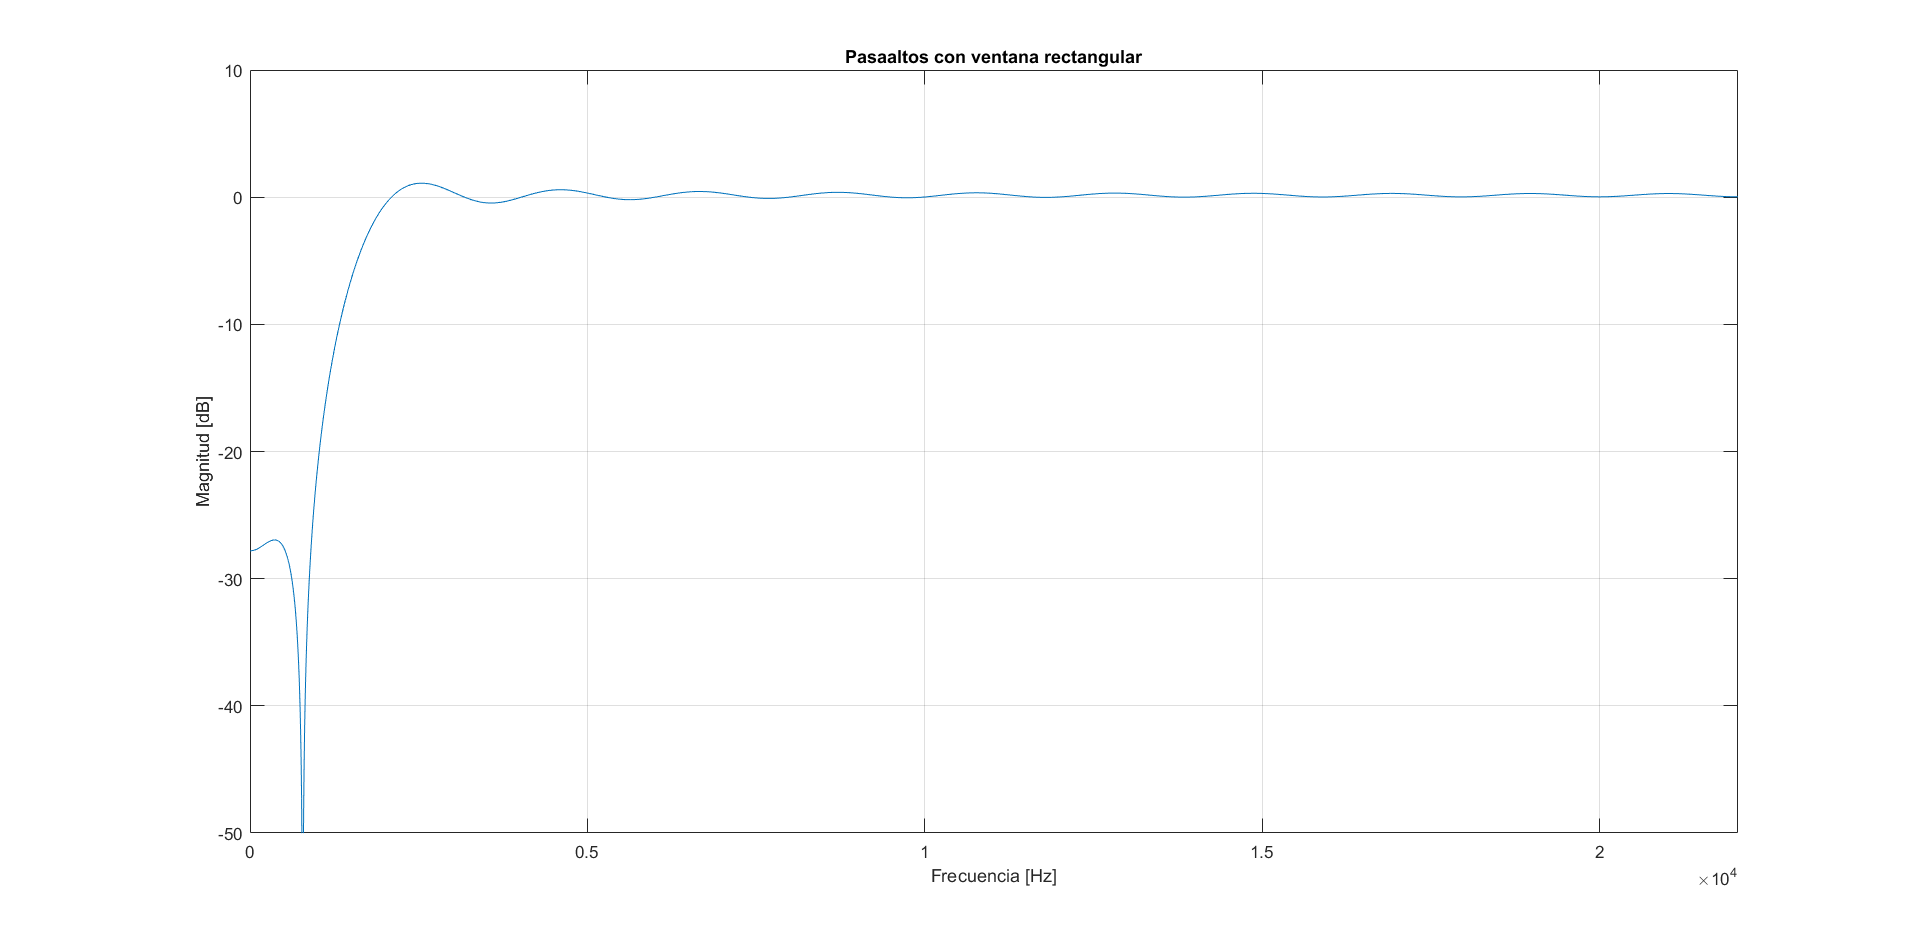
\includegraphics[scale=.35]{./images/1/recmod.png}
  \caption{Respuesta en frecuencia del pasaaltos con ventana rectangular.}
\end{figure}
\begin{figure}[H]
  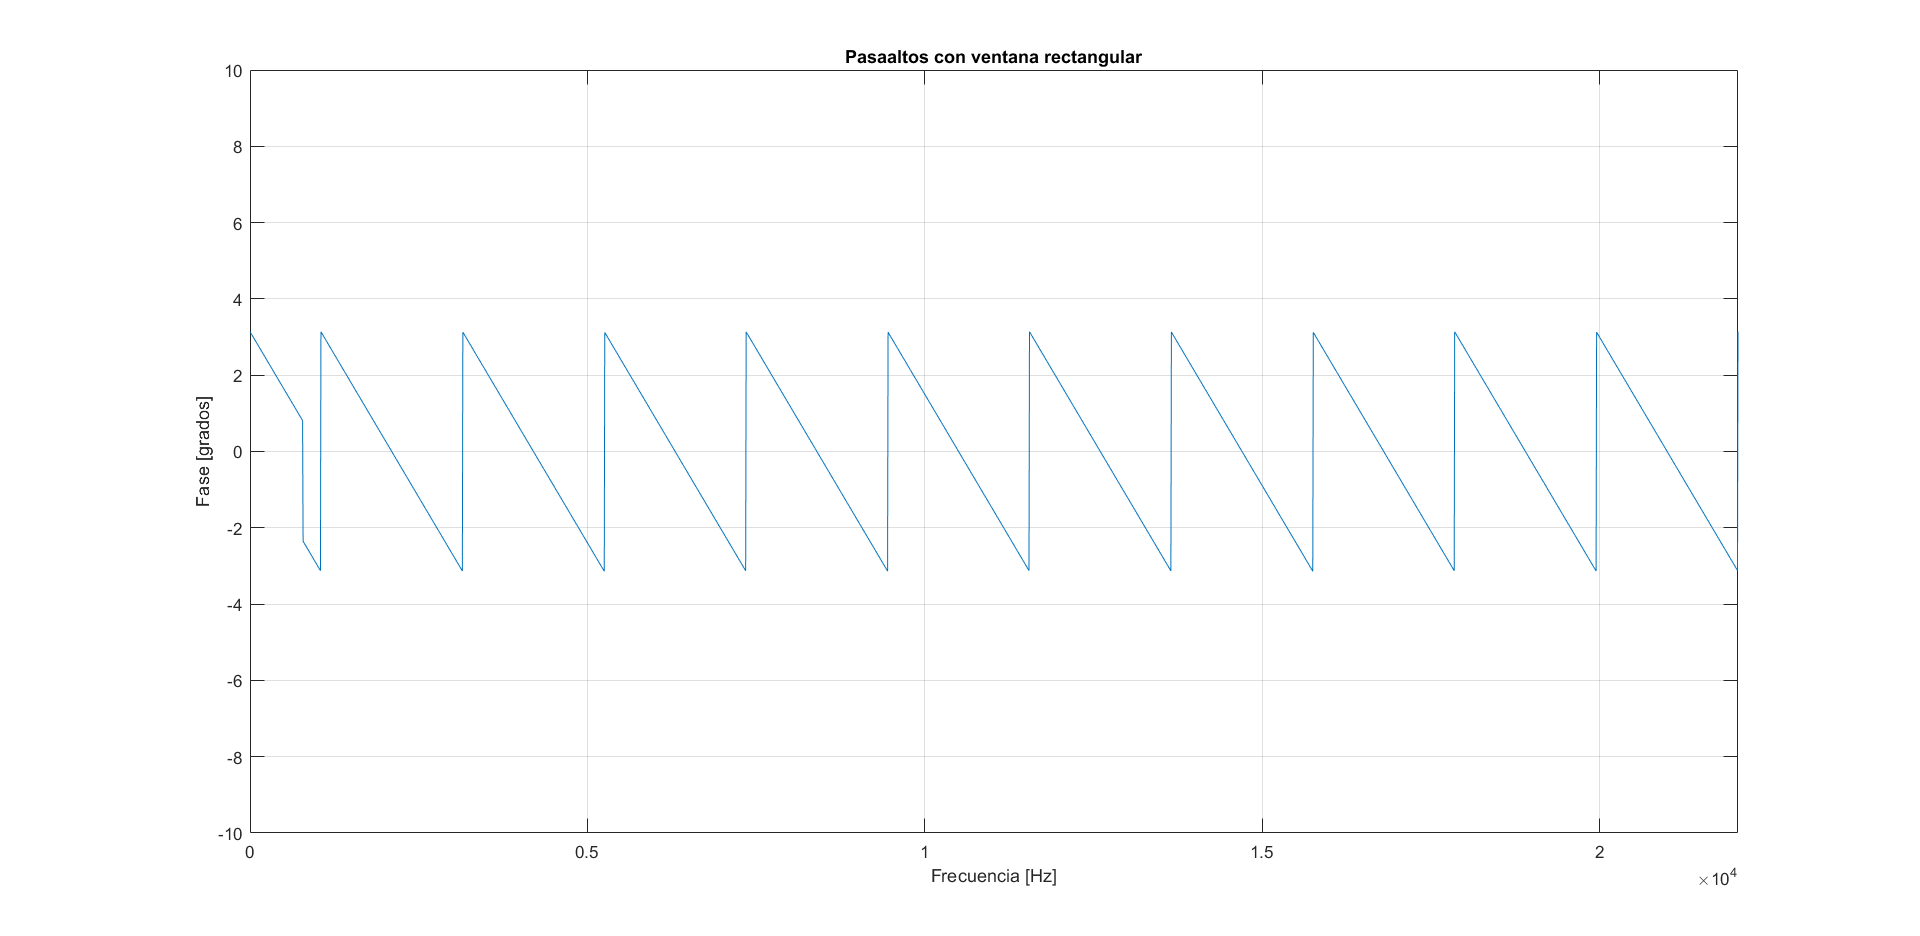
\includegraphics[scale=.35]{./images/1/recfase.png}
  \caption{Fase del pasaaltos con ventana rectangular.}
\end{figure}

\subsection{Ventana de Hamming}
La ventana de Hamming está definida por:
\begin{equation}
    \omega (n+1)=0.54+0.46\cos\left(\frac{2\pi n}{N-1} \right)  \qquad  0<n<N-1
\end{equation}
\begin{figure}[H]
  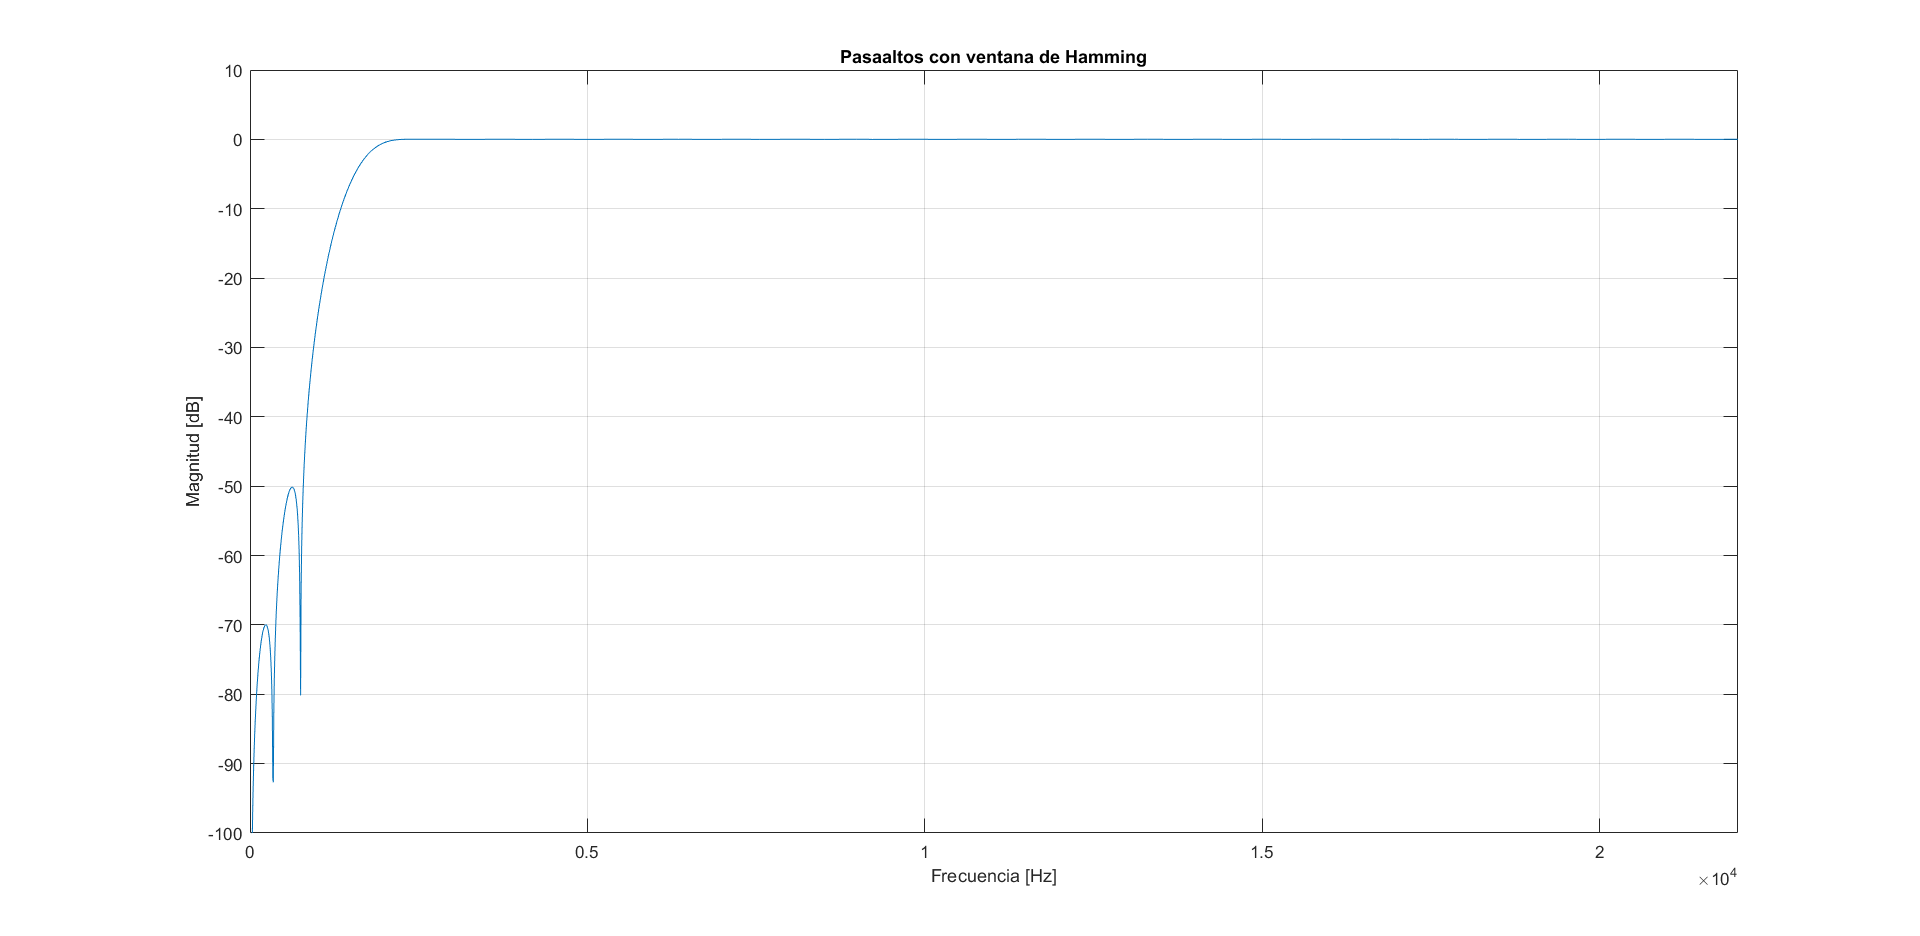
\includegraphics[scale=.35]{./images/1/hammingmod.png}
  \caption{Respuesta en frecuencia del pasaaltos con ventana de Hamming.}
\end{figure}
\begin{figure}[H]
  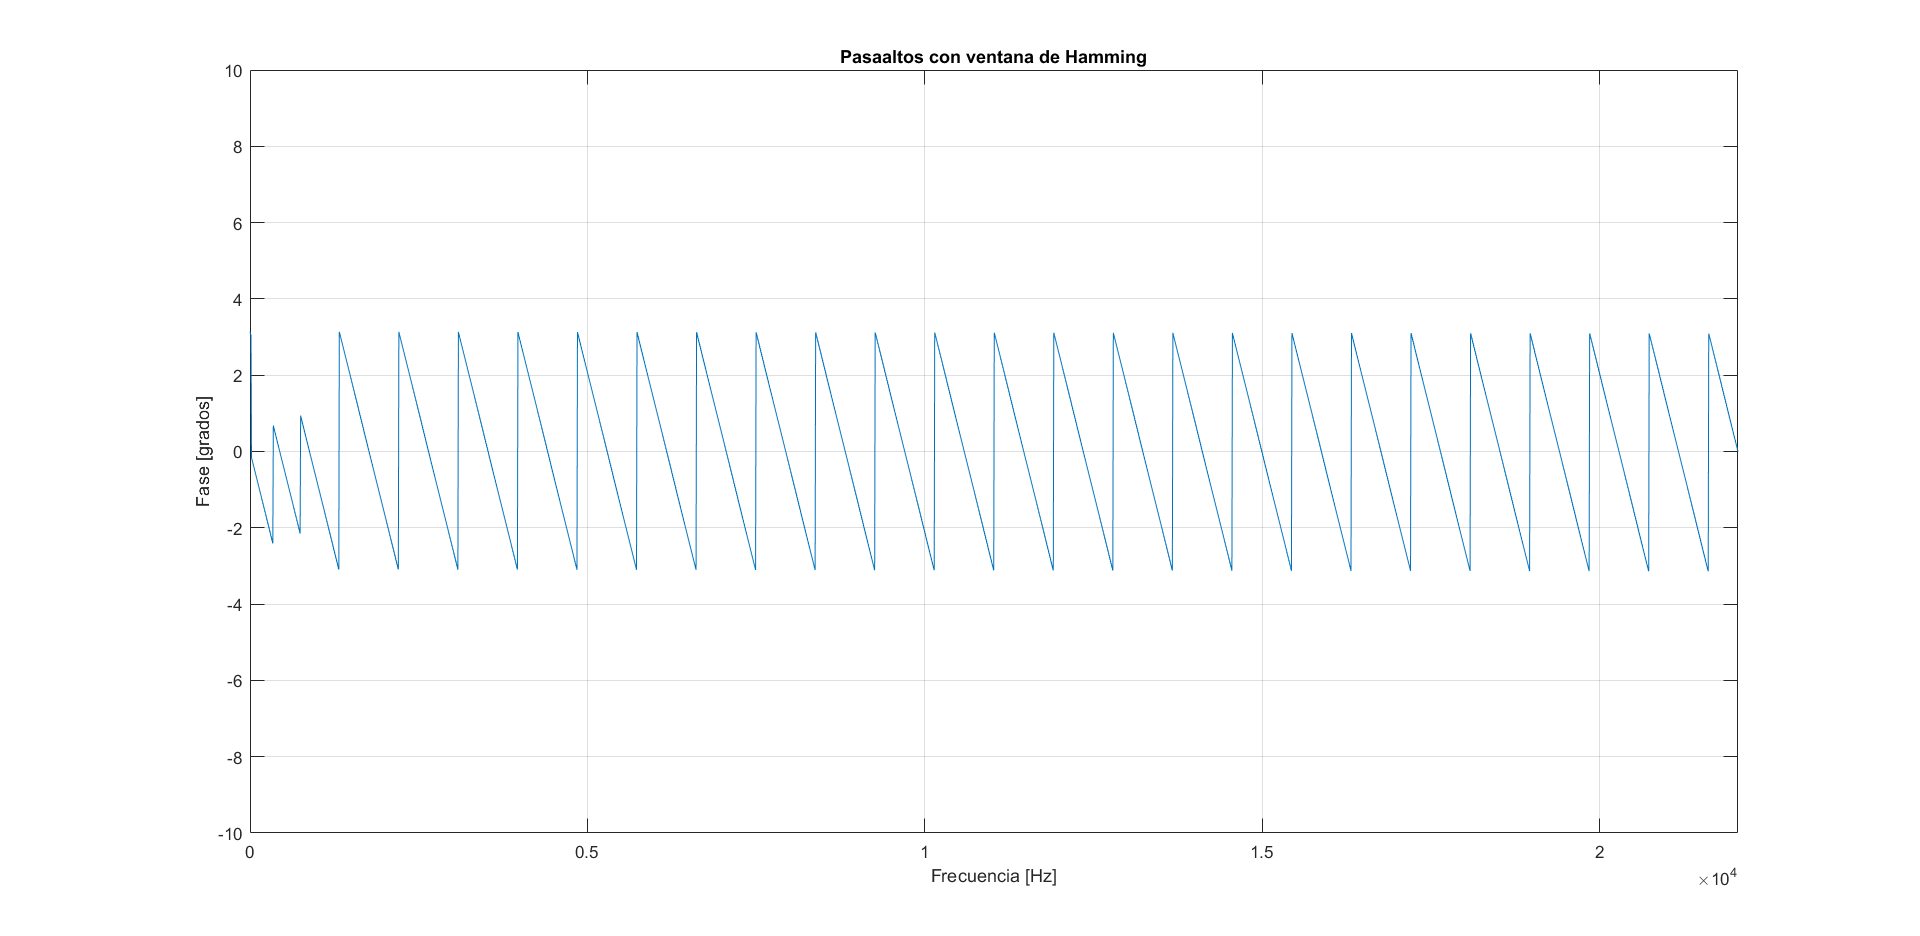
\includegraphics[scale=.35]{./images/1/hammingfase.png}
  \caption{Fase del pasaaltos con ventana de Hamming.}
\end{figure}
